\section{Analysis}\label{sec:analysis}

% Figure plan: notes/figure_guide.md §2. Qualitative scenes come from recorded dumps only
% (path + md5 in the figure source note) and the selection rule is stated in the caption.

\subsection{Where Sensor Over-Reliance Comes From}
A fusion model can lean on one sensor because its architecture or supervision favours that sensor, or because the training data make that sensor sufficient. DGFusion~\cite{dgfusion2026} is a useful test case: it adds depth supervision to its fusion, and removing depth costs our reproduction of DGFusion 23 to 37 points depending on the condition (Fig.~\ref{fig:dependence}). If the depth supervision caused this dependence, a model without it should behave differently.

Our own model trained without C2D2, which has no depth supervision, shows the same pattern: removing depth costs 23.5 to 38.7 points, and the cost grows from sun to low exposure as for DGFusion. The same architecture trained with C2D2 loses only 3.9 points in sun, 10.1 at night, and 13.4 under low exposure. The effect also appears in a second architecture: when we re-train DGFusion with the same synthetic degradation, removing depth entirely costs 4.7 points, whereas it costs 33.3 points for our reproduction trained without degradation and 33.4 for the official weights (Table~\ref{tab:robust}).
% Sources: judgment-ledger:112 (2026-09-30 row: E1 confirmed, Q2 s821, DGFusion reproduction (a), oracle_cond probe);
% judgment-ledger:117 (reproduction (a) -> retrained (b): depth fully missing -33.3 -> -4.7); judgment-ledger:130 (official weights -33.4).

These measurements suggest that, on DELIVER, the dependence on depth comes mainly from training without degraded sensors rather than from a particular fusion design or supervision \todo{final wording after FU-04 (C2D2 applied to DGFusion and CAFuser) and FU-05 (all curves on one split)}. A plausible reason is that DELIVER renders depth without noise or holes, so training on complete inputs finds a shortcut that real depth sensors would not offer. The comparison has two caveats: the model trained without C2D2 was trained for 200 epochs and the C2D2 model for 40, and the DGFusion curve was measured on the test split while ours were measured on validation. A complementary observation is that our model trained without C2D2 is already less sensitive to salt-and-pepper noise than the re-trained DGFusion; we therefore attribute part of the noise robustness to the frozen DINOv3 backbone rather than to C2D2 \todo{state the measured drops (ledger:117: E1 3.09/5.73/11.22 vs DGFusion retrained 5.9/14.3/31.4) after checking that the definitions match}.

\begin{figure}[t]
\centering
% Source numbers and provenance: figures/src/make_data_figs.py (fig_dependence). Full table: sections/supp_tables.tex (Table S1).
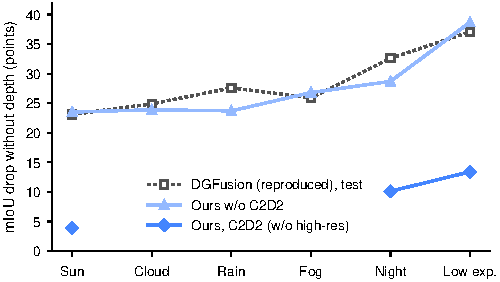
\includegraphics[width=\columnwidth]{figures/fig_dependence.pdf}
\caption{Drop in mIoU when depth is removed, per condition. Our model trained without C2D2 relies on depth as heavily as our reproduction of DGFusion, whose design adds depth supervision; the same architecture trained with C2D2 loses much less. DGFusion was measured on test, the other curves on val. \todo{re-measure all curves on one split; add the full model and the retrained baselines.}}
\label{fig:dependence}
\end{figure}

\subsection{What the High-Resolution Path Adds}
The high-resolution path raises clean test mIoU by 1.15 points on average over three seeds (from 56.59 to 57.74; Table~\ref{tab:robust}). Fig.~\ref{fig:thin} shows where the gain comes from. Averaged over the three seeds, Static gains 10.4 points, Pedestrian 3.8, TrafficSign 3.1, and Pole 2.1, and the four thin classes gain 3.0 points together. The gain comes mainly from recall: for Pole the recall rises from 0.75 to 0.78 and for Pedestrian from 0.89 to 0.90 \todo{confirm these recall values (two seeds, NAS analysis\_logs/a2\_thin\_anatomy\_20261018/summary.md) through the analysis session before citing}. Two classes lose: TrafficLight by 4.1 points and RailTrack by 7.2. RailTrack varies strongly between seeds even without the path (58.5, 32.6, and 45.1 for the three seeds), so we do not interpret its change. The TrafficLight loss, in contrast, is systematic and is analysed next.
% Sources: per-class 3-seed CSV .claude_logs/experiments/analysis/DRN-261018-01/a2_vs_q2_perclass_3seed.csv (d_mean3 column);
% thin-4 mean +3.04 and 24-class Δ +1.50: tasks/DRN-261018-01/analysis.md.

\begin{figure}[t]
\centering
% Source: .claude_logs/experiments/analysis/DRN-261018-01/a2_vs_q2_perclass_3seed.csv (3 seeds, legal v2 test 1024);
% plot: figures/src/make_data_figs.py (fig_thin).
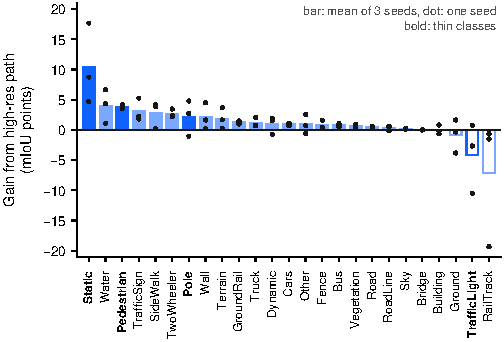
\includegraphics[width=\columnwidth]{figures/fig_thin.pdf}
\caption{Per-class gain of the high-resolution path on DELIVER test, paired by seed (full model minus the same model without the path). Thin classes gain most; TrafficLight and RailTrack lose and vary strongly across seeds. \todo{add zoomed crops of thin objects (Q2 dumps on yeon).}}
\label{fig:thin}
\end{figure}

\subsection{Failure Case: Posters Read as Traffic Lights}
With the high-resolution path, the recall of TrafficLight rises (0.80 to 0.85) but its precision falls (0.46 to 0.41) \todo{same confirmation as above}. Fig.~\ref{fig:failure} shows where the extra false positives appear. In the scenes with the largest increase, billboards and posters, labelled as \emph{Other}, are painted as traffic lights, and in one rainy scene a traffic sign is. The two classes share fine structure, a small bright rectangular shape on a pole or a wall, but differ in context. Because the high-resolution features are added to every pyramid level without a gate, fine detail reaches the dense per-pixel classifier directly, and the classifier can follow the detail without enough context. This mechanism is a hypothesis that our measurements are consistent with but do not prove; we discuss a remedy in Section~\ref{sec:conclusion}.
% Source: NAS analysis_logs/a2_tl_fp_scenes_20261022/README.md (4 scenes; A2 vs Q2 TrafficLight FP pixels
% 15258 vs 3620, 13705 vs 3752, 10304 vs 2008, 12229 vs 9008; selection rule: top-20 by A2 FP - Q2 FP, no repeated condition).

\begin{figure}[t]
\centering
% Assets: NAS analysis_logs/a2_tl_fp_scenes_20261022 (4 scenes, README.md has the selection rule).
\phbox{4.2cm}{limitation: posters and signs predicted as traffic light (2 of the 4 recorded scenes; RGB, ground truth, ours, error map)}
\caption{\todo{caption; selection rule from the scene README: among the 20 test images where our model adds the most TrafficLight false positives relative to the model without the high-resolution path, one scene per condition.}}
\label{fig:failure}
\end{figure}

\subsection{Limitations}
First, DELIVER is synthetic, and its complete depth is the reason the shortcut exists; the size of the effect on real depth sensors remains to be measured, and MUSES does not contain depth. Second, all our runs use a 40-epoch schedule and three seeds, while the baselines are single runs, so differences below about one point should not be over-read. Third, the high-resolution path makes the model slightly more sensitive to the strongest pixel noise than the same model without it (47.85 vs.\ 48.79, Table~\ref{tab:robust}); a likely cause is that its convolutional stem sees raw pixels, which we have not yet verified. Fourth, a single shared LoRA reached the same clean accuracy as sensor-specific adapters in one seed (Table~\ref{tab:ablation}); \todo{update once the shared-LoRA robustness test decides which variant is the paper model}.
